\documentclass{beamer}
\usepackage[maxbibnames=99]{biblatex}
\usepackage{calc}
\usepackage[T1]{fontenc}
\usepackage{graphicx}
\usepackage{listings}
\usepackage{multicol}
\usepackage{textcomp}
\usepackage{tikz}
\usepackage{verbatim}
\usepackage{xcolor}

\addbibresource{siamCseTalk.bib}

%
%  Options list:
%
%   strictfont - use Sandia Corporate-specified font (Calibri).  Omit if you don't
%      care about using Calibri or don't have it installed.
%   theme - select theme.  Choose from blue,white,sand,left,right.  Try it!
%   slidenumber - include slide numbers on body slides
%   slidedate - include date on body slides
%   titledate - include date on title slide
%

\mode<presentation>
{
  \usetheme[strictfont,theme=sand,slidenumber,titledate]{Sandia}
}

\title{Panzer}
\subtitle{A Finite Element Assembly Engine within the Trilinos Framework}
\author[Jason Gates]{\emph{Jason M. Gates}, Roger P. Pawlowksi, Eric C. Cyr\\\footnotesize\emph{Sandia National Laboratories}}
\date{March 3, 2017}

%
%  Use this macro to turn on OUO markings and provide the appropriate OUO information
%  Options include:
%    exemption - numeric (2-9) indicator of which FOIA exemption this material falls under
%       The template will supply the text.
%    nameorg - OUO name and organization, as a string
%    date - OUO date, defaults to \insertdate
%    guidance - Any OUO guidance to include on the marking
%
%\sandiabeamerMarkOUO{exemption=3,nameorg=Patrick M. Widener (1423)}

%
% Use this macro to specify the SAND number of your presentation
%
\sandiabeamerSANDInfo{number=2017-1977 C}

\setbeamercovered{transparent}

\newcommand{\Grad}[1]{\nabla #1}
\newcommand{\Div}[1]{\nabla \cdot #1}
\newcommand{\Del}[2]{\frac{\partial #1}{\partial #2}}

\usetikzlibrary{arrows}
\usetikzlibrary{graphs}
\usetikzlibrary{graphdrawing}
\usetikzlibrary{positioning}
\usegdlibrary{layered}

\lstset{
  language=C++,
  upquote=true,
  basicstyle=\ttfamily\scriptsize,
  commentstyle=\color{blue!80!black},
  stringstyle=\color{red!80!black},
  showstringspaces=false,
  breaklines=true,
  breakatwhitespace=true,
  breakindent=0pt,
  postbreak=\space\space,
  emph={[1]template,typename,class,void,string,int,vector,double,const,typedef,auto},
  emphstyle={[1]\color{green!80!black}},
  emph={[2]panzer,std,Teuchos,PHX,Kokkos},
  emphstyle={[2]\color{red!70}},
  emph={[3]public,private,this,new,for},
  emphstyle={[3]\color{orange!80!black}}
}

\renewcommand{\vdots}{\tikz[baseline,every node/.style={inner sep=0}]{\node at (0,0){.};\node at (0,2pt){.};\node at (0,4pt){.};}}

\newcommand{\cbox}[2]{\setlength{\fboxsep}{1pt}\colorbox{#1}{#2}}
\newcommand{\redbox}[1]{\cbox{red!50}{#1}}
\newcommand{\orangebox}[1]{\cbox{orange!50}{#1}}
\newcommand{\greenbox}[1]{\cbox{green!50}{#1}}
\newcommand{\bluebox}[1]{\cbox{cyan!50}{#1}}

\renewcommand*{\bibfont}{\fontsize{7}{9}\selectfont}
\setbeamertemplate{bibliography item}{\insertbiblabel}

\begin{document}

\begin{frame}
  \titlepage
\end{frame}

\section{What is Panzer?}

  \begin{frame}
    \frametitle{What is Panzer?}
    \begin{itemize}
      \item C++ Library
      \item General finite element assembly engine for multi-physics
            simulation
      \item Supports 1-, 2-, \& 3-D unstructured mesh calculations
      \item Supplies quantities needed for advanced \alert{solution} and
            \alert{analysis} algorithms
            \begin{itemize}
              \item residuals
              \item Jacobians
              \item parameter sensitivities
              \item stochastic residuals/etc.
            \end{itemize}
    \end{itemize}
  \end{frame}

  \begin{frame}
    \frametitle{What is Panzer?}
    \begin{itemize}
      \item Contains no physics-specific code---physics applications are
            light-weight front ends
      \item Massively parallel for complex physics
      \item Leverages template-based generic programming\cite{sacado} to assemble quantities of interest
      \item Incorporates 35 Trilinos packages
    \end{itemize}
  \end{frame}

  \begin{frame}
    \frametitle{What is Panzer \alert{not}?}
    \begin{itemize}
      \item Application
      \item Domain specific language
      \item Front end preprocessor/interpreter
      \item deal.II, FEniCS, MFEM, MOOSE, Sundance
    \end{itemize}
  \end{frame}

  \begin{frame}
    \frametitle{Panzer's History}
    \begin{itemize}
      \item Lessons learned from Sandia's PDE physics codes
      \begin{itemize}
        \item Charon1, MPSalsa, etc.
      \end{itemize}
      \item Monolithic application $\longrightarrow$ library of packages
      \item Capabilities explored/developed $\longrightarrow$ Phalanx, Panzer
    \end{itemize}
    \begin{figure}
      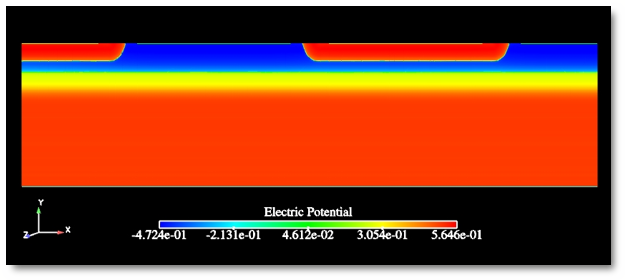
\includegraphics[height=.4\textheight]{driftDiffusion}
    \end{figure}
  \end{frame}

  \begin{frame}
    \frametitle{Panzer's History}
    \begin{itemize}
      \item Drekar:  advanced algorithm demonstration
      \item Applications (Drekar, Charon2, EMPIRE, etc.) drive Panzer's requirements, design goals
      \begin{itemize}
        \item Coupled multi-physics
        \item Large scale simulation (>100k cores)
        \item Finite element focussed (currently)
        \item Embedded analysis (AD, sensitivities)
        \item Technology sharing and deployment
      \end{itemize}
      \item Panzer provides applications with flexible infrastructure, core technologies
    \end{itemize}
  \end{frame}

  \begin{frame}
    \frametitle{Panzer Enables}
    \begin{columns}
      \begin{column}{0.6\textwidth}
        \begin{itemize}
          \item Applications
          \begin{itemize}
            \item Turbulent CFD
            \item Magnetohydrodynamics
            \item Semiconductor devices
          \end{itemize}
          \item Supporting technologies
          \begin{itemize}
            \item Algebraic multigrid
            \item Block preconditioning
            \item Uncertainty quantification
            \item IMEX
            \item PDE constrained optimization
            \item Compatible discretizations
          \end{itemize}
        \end{itemize}
      \end{column}
      \begin{column}{0.4\textwidth}
        \begin{tabular}{c}
          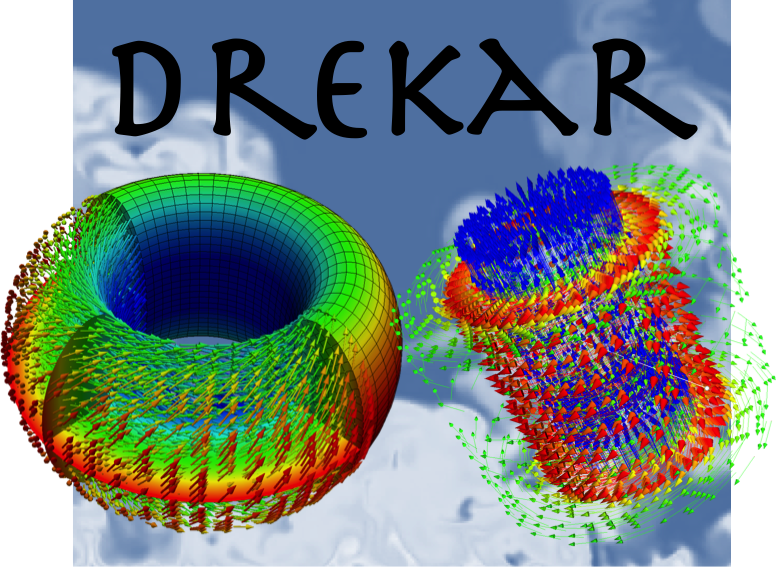
\includegraphics[width=.9\textwidth]{drekarLogo}\\
          \ \,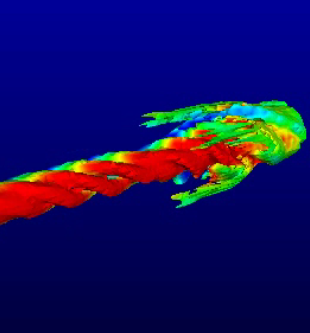
\includegraphics[width=.7\textwidth]{turbulentCfd}
        \end{tabular}
      \end{column}
    \end{columns}
  \end{frame}

\section{How does it work?}

  \begin{frame}
    \frametitle{Element \& Physics Blocks}
    \begin{figure}
      \begin{tikzpicture}[scale=0.8]
        \filldraw[red!80!black,opacity=0.5] (0,0) rectangle (4,4);
        \filldraw[green!80!black,opacity=0.5] (4,0) rectangle (8,4);
        \draw[step=1cm,black,very thin,opacity=0.5] (0,0) grid (8,4);
        \draw (2,0) node[below,red!80!black] {Element Block 0};
        \draw (6,0) node[below,green!80!black] {Element Block 1};
        \draw (2,2) node[align=center,fill=red!40!white,rounded corners=2pt] {Solid\\Physics\\Block};
        \draw (6,2) node[align=center,fill=green!40!white,rounded corners=2pt] {Fluid\\Physics\\Block};
      \end{tikzpicture}
    \end{figure}
    \begin{itemize}
      \item Users divide the domain into \alert{element blocks}
      \item Each element block maps to a single \alert{physics block}
      \item Physics blocks contain a list of \alert{equation sets}
    \end{itemize}
  \end{frame}

  \begin{frame}
    \frametitle{Equation Sets}
    \begin{figure}
      \begin{tikzpicture}[scale=0.6,remember picture]
        \filldraw[red!80!black,opacity=0.5] (0,0) rectangle (4,4);
        \filldraw[green!80!black,opacity=0.5] (4,0) rectangle (8,4);
        \draw[step=1cm,black,very thin,opacity=0.5] (0,0) grid (8,4);
        \draw (2,2) node[fill=red!40!white,rounded corners=2pt] {Solid};
        \draw (6,2) node[fill=green!40!white,rounded corners=2pt] {Fluid};
        \draw (0,2) node (solid) {};
        \draw (8,3) node (fluidTop) {};
        \draw (8,1) node (fluidBottom) {};
      \end{tikzpicture}
    \end{figure}
    \begin{itemize}
      \item Equation sets define the form of the PDE
      \item Details are filled in using \alert{closure models}
    \end{itemize}
    \begin{description}
      \item[Navier-Stokes]
      \begin{tabular}{c}
        $\displaystyle\Del{u}{t} + u \cdot \Grad{u} - \Div{(\alert{\nu} \Grad{u})} + \Grad{p} = \alert{f}$\\
        $\Div{u} = 0$
      \end{tabular}
      \tikz[remember picture] \node (navierStokes) {};
      \item[Energy]
      \tikz[remember picture] \node (energyLeft) {};
      $\displaystyle\Del{T}{t} + u \cdot \Grad{T} - \Div{(\alert{\sigma} \Grad{T})} = 0$
      \tikz[remember picture] \node (energyRight) {};
    \end{description}
    \begin{tikzpicture}[remember picture,overlay]
      \draw[->,>=stealth',very thick,green!80!black] (navierStokes) -- +(1,0) |- (fluidBottom);
      \draw[->,>=stealth',very thick,green!80!black] (energyRight) -- +(3,0) |- (fluidTop);
      \draw[->,>=stealth',very thick,red!80!black] (energyLeft) +(-1.5,0) -- +(-2.5,0) |- (solid);
    \end{tikzpicture}
  \end{frame}

  \begin{frame}
    \frametitle{Data Mapping Utilities}
    Finite element discretizations have changed
    \begin{itemize}
      \item Historically used nodal equal-order finite elements
      \item New code embraces mixed discretizations
      \item Also using high-order compatible discretizations
      \item \textcolor{red!80!black}{$H_{grad}$} (nodal), \textcolor{green!80!black}{$H_{curl}$} (edge), \textcolor{blue!80!black}{$H_{div}$} (face)
      \item Requires extra data management (orientations)
    \end{itemize}
    \begin{figure}
      \begin{tikzpicture}[scale=1.5]
        \foreach \x in {0,2,4}
          \draw (\x,0) rectangle (\x+1,1);
        \foreach \x in {0,1}
          \foreach \y in {0,1}
            \filldraw (\x,\y) circle[radius=1.5pt];
        \draw[->,>=stealth',very thick] (2.1,0) -- (2.9,0);
        \draw[->,>=stealth',very thick] (3,0.1) -- (3,0.9);
        \draw[->,>=stealth',very thick] (2.9,1) -- (2.1,1);
        \draw[->,>=stealth',very thick] (2,0.9) -- (2,0.1);
        \draw[->,>=stealth',very thick] (4,0.5) -- (3.7,0.5);
        \draw[->,>=stealth',very thick] (4.5,0) -- (4.5,-0.3);
        \draw[->,>=stealth',very thick] (5,0.5) -- (5.3,0.5);
        \draw[->,>=stealth',very thick] (4.5,1) -- (4.5,1.3);
        \draw (0.5,0.5) node[red!80!black] {$H_{grad}$};
        \draw (2.5,0.5) node[green!80!black] {$H_{curl}$};
        \draw (4.5,0.5) node[blue!80!black] {$H_{div}$};
      \end{tikzpicture}
    \end{figure}
  \end{frame}

  \begin{frame}
    \frametitle{Data Mapping Utilities}
    Three primary pieces:\\
    \begin{description}
      \item[FieldPattern\ \ \ ]  \ Describes basis layout \& continuity of
                                 fields
      \item[ConnManager]         Mesh topology from field pattern (mesh
                                 abstraction)
      \item[DOFManager]          \ \,Manages and computes unknown field numbers
    \end{description}
    \begin{itemize}
      \item \alert{Panzer = mesh-agnostic}
      \item panzer\_stk = concrete implementation of ConnManager
    \end{itemize}
  \end{frame}

  \begin{frame}[t]
    \frametitle{FieldPattern}
    \begin{description}
      \item[Linear]     \alert<2>{pressure}, \alert<2>{temperature}
      \item[Quadratic]  \alert<3>{velocities}
    \end{description}
    \begin{figure}
      \begin{tikzpicture}[scale=2]
        \draw[white] (0,0) circle[radius=1pt] (5,1) circle[radius=1pt];
        \draw[white] (1.5,0) node[below=1ex] {$u_x,u_y,p,T$};
        \only<2->
        {
          \draw (0,0) rectangle (1,1);
          \foreach \x in {0,1}
            \foreach \y in {0,1}
              \filldraw (\x,\y) circle[radius=1pt];
          \draw (0.5,0) node[below=1ex] {$p,T$};
        }
        \only<3->
        {
          \draw (2,0) rectangle (3,1);
          \foreach \x in {2,2.5,3}
            \foreach \y in {0,0.5,1}
              \filldraw (\x,\y) circle[radius=1pt];
          \draw (2.5,0) node[below=1ex] {$u_x,u_y$};
        }
        \only<4>
        {
          \draw (4,0) rectangle (5,1);
          \foreach \x in {4,4.5,5}
            \foreach \y in {0,0.5,1}
              \filldraw (\x,\y) circle[radius=1pt];
          \draw (4.5,0) node[below=1ex] {$u_x,u_y,p,T$};
          \draw (1.5,0.5) node {\Huge$\bigcup$};
          \draw (3.5,0.5) node {\Huge$=$};
        }
      \end{tikzpicture}
      \begin{tabular}{c}
        $\displaystyle\Del{\alert<3>{u}}{t} + \alert<3>{u} \cdot \Grad{\alert<3>{u}} - \Div{(\nu \Grad{\alert<3>{u}})} + \Grad{\alert<2>{p}} = f$\\
        $\Div{\alert<3>{u}} = 0$\\
        $\displaystyle\Del{\alert<2>{T}}{t} + \alert<3>{u} \cdot \Grad{\alert<2>{T}} - \Div{(\sigma \Grad{\alert<2>{T}})} = 0$
      \end{tabular}
    \end{figure}
  \end{frame}

  \begin{frame}[t]
    \frametitle{ConnManager}
    \begin{description}
      \item[Linear]     pressure, temperature
      \item[Quadratic]  velocities
    \end{description}
    \begin{figure}
      \begin{tikzpicture}[scale=1.6]
        \filldraw[red!80!black,opacity=0.5] (0,0) rectangle (2,2);
        \filldraw[green!80!black,opacity=0.5] (2,0) rectangle (4,2);
        \draw[step=1cm,black,very thin,opacity=0.5] (0,0) grid (4,2);
        \draw (1,0) node[red!80!black,below=4pt] {Solid ($T$)};
        \draw (3,0) node[green!80!black,below=4pt] {Fluid ($u_x,u_y,p,T$)};
        \foreach \x in {0,0.5,...,4}
          \foreach \y in {0,0.5,...,2}
            \filldraw (\x,\y) circle[radius=1pt];
        \draw (2,-0.65) node {Numbering = mesh topology};
        \draw (0.0,2.0) node[above right=-2pt] {\tiny  0};
        \draw (1.0,2.0) node[above right=-2pt] {\tiny  1};
        \draw (2.0,2.0) node[above right=-2pt] {\tiny  2};
        \draw (0.0,1.0) node[above right=-2pt] {\tiny  3};
        \draw (1.0,1.0) node[above right=-2pt] {\tiny  4};
        \draw (2.0,1.0) node[above right=-2pt] {\tiny  5};
        \draw (0.0,0.0) node[above right=-2pt] {\tiny  6};
        \draw (1.0,0.0) node[above right=-2pt] {\tiny  7};
        \draw (2.0,0.0) node[above right=-2pt] {\tiny  8};
        \draw (3.0,2.0) node[above right=-2pt] {\tiny  9};
        \draw (4.0,2.0) node[above right=-2pt] {\tiny 10};
        \draw (3.0,1.0) node[above right=-2pt] {\tiny 11};
        \draw (4.0,1.0) node[above right=-2pt] {\tiny 12};
        \draw (3.0,0.0) node[above right=-2pt] {\tiny 13};
        \draw (4.0,0.0) node[above right=-2pt] {\tiny 14};
        \draw (0.5,2.0) node[above right=-2pt] {\tiny 15};
        \draw (1.5,2.0) node[above right=-2pt] {\tiny 16};
        \draw (0.0,1.5) node[above right=-2pt] {\tiny 17};
        \draw (1.0,1.5) node[above right=-2pt] {\tiny 18};
        \draw (2.0,1.5) node[above right=-2pt] {\tiny 19};
        \draw (0.5,1.0) node[above right=-2pt] {\tiny 20};
        \draw (1.5,1.0) node[above right=-2pt] {\tiny 21};
        \draw (0.0,0.5) node[above right=-2pt] {\tiny 22};
        \draw (1.0,0.5) node[above right=-2pt] {\tiny 23};
        \draw (2.0,0.5) node[above right=-2pt] {\tiny 24};
        \draw (0.5,0.0) node[above right=-2pt] {\tiny 25};
        \draw (1.5,0.0) node[above right=-2pt] {\tiny 26};
        \draw (2.5,2.0) node[above right=-2pt] {\tiny 27};
        \draw (3.5,2.0) node[above right=-2pt] {\tiny 28};
        \draw (3.0,1.5) node[above right=-2pt] {\tiny 29};
        \draw (4.0,1.5) node[above right=-2pt] {\tiny 30};
        \draw (2.5,1.0) node[above right=-2pt] {\tiny 31};
        \draw (3.5,1.0) node[above right=-2pt] {\tiny 32};
        \draw (3.0,0.5) node[above right=-2pt] {\tiny 33};
        \draw (4.0,0.5) node[above right=-2pt] {\tiny 34};
        \draw (2.5,0.0) node[above right=-2pt] {\tiny 35};
        \draw (3.5,0.0) node[above right=-2pt] {\tiny 36};
        \draw (0.5,1.5) node[above right=-2pt] {\tiny 37};
        \draw (1.5,1.5) node[above right=-2pt] {\tiny 38};
        \draw (0.5,0.5) node[above right=-2pt] {\tiny 39};
        \draw (1.5,0.5) node[above right=-2pt] {\tiny 40};
        \draw (2.5,1.5) node[above right=-2pt] {\tiny 41};
        \draw (3.5,1.5) node[above right=-2pt] {\tiny 42};
        \draw (2.5,0.5) node[above right=-2pt] {\tiny 43};
        \draw (3.5,0.5) node[above right=-2pt] {\tiny 44};
      \end{tikzpicture}
    \end{figure}
  \end{frame}

  \begin{frame}[t]
    \frametitle{DOFManager\cite{dofManager}}
    \begin{description}
      \item[Linear]     pressure, temperature
      \item[Quadratic]  velocities
    \end{description}
    \begin{tikzpicture}[remember picture,overlay]
      \node at ([yshift=-2.4ex]current page.center)
      {
        \begin{tikzpicture}[scale=1.6]
          \filldraw[red!80!black,opacity=0.1] (0,0) rectangle (2,2);
          \filldraw[green!80!black,opacity=0.1] (2,0) rectangle (4,2);
          \draw[step=1cm,black,very thin,opacity=0.2] (0,0) grid (4,2);
          \draw (1,0) node[red!80!black,below=4pt] {Solid ($\textcolor{cyan}{T}$)};
          \draw (3,0) node[green!80!black,below=4pt] {Fluid ($\textcolor{red!80!black}{u_x},\textcolor{orange}{u_y},\textcolor{green!80!black}{p},\textcolor{cyan}{T}$)};
          \foreach \x in {0,1}
            \foreach \y in {0,1,2}
              \filldraw (\x,\y) circle[radius=1pt];
          \foreach \x in {2,2.5,...,4}
            \foreach \y in {0,0.5,...,2}
              \filldraw (\x,\y) circle[radius=1pt];
          \draw (2,-0.65) node {Unknown field numbering};
          \draw (0.0,2.0) node[above=-2pt,rotate=30] {\tiny \bluebox{0}};
          \draw (1.0,2.0) node[above=-2pt,rotate=30] {\tiny \bluebox{1}};
          \draw (2.0,2.0) node[above=-2pt,rotate=30] {\tiny \redbox{2},\orangebox{3},\greenbox{4},\bluebox{5}};
          \draw (0.0,1.0) node[above=-2pt,rotate=30] {\tiny \bluebox{6}};
          \draw (1.0,1.0) node[above=-2pt,rotate=30] {\tiny \bluebox{7}};
          \draw (2.0,1.0) node[above=-2pt,rotate=30] {\tiny \redbox{8},\orangebox{9},\greenbox{10},\bluebox{11}};
          \draw (0.0,0.0) node[above=-2pt,rotate=30] {\tiny \bluebox{12}};
          \draw (1.0,0.0) node[above=-2pt,rotate=30] {\tiny \bluebox{13}};
          \draw (2.0,0.0) node[above=-2pt,rotate=30] {\tiny \redbox{14},\orangebox{15},\greenbox{16},\bluebox{17}};
          \draw (3.0,2.0) node[above=-2pt,rotate=30] {\tiny \redbox{18},\orangebox{19},\greenbox{20},\bluebox{21}};
          \draw (4.0,2.0) node[above=-2pt,rotate=30] {\tiny \redbox{22},\orangebox{23},\greenbox{24},\bluebox{25}};
          \draw (3.0,1.0) node[above=-2pt,rotate=30] {\tiny \redbox{26},\orangebox{27},\greenbox{28},\bluebox{29}};
          \draw (4.0,1.0) node[above=-2pt,rotate=30] {\tiny \redbox{30},\orangebox{31},\greenbox{32},\bluebox{33}};
          \draw (3.0,0.0) node[above=-2pt,rotate=30] {\tiny \redbox{34},\orangebox{35},\greenbox{36},\bluebox{37}};
          \draw (4.0,0.0) node[above=-2pt,rotate=30] {\tiny \redbox{38},\orangebox{39},\greenbox{40},\bluebox{41}};
          \draw (2.0,1.5) node[above=-2pt,rotate=30] {\tiny \redbox{42},\orangebox{43}};
          \draw (2.0,0.5) node[above=-2pt,rotate=30] {\tiny \redbox{44},\orangebox{45}};
          \draw (2.5,2.0) node[above=-2pt,rotate=30] {\tiny \redbox{46},\orangebox{47}};
          \draw (3.5,2.0) node[above=-2pt,rotate=30] {\tiny \redbox{48},\orangebox{49}};
          \draw (3.0,1.5) node[above=-2pt,rotate=30] {\tiny \redbox{50},\orangebox{51}};
          \draw (4.0,1.5) node[above=-2pt,rotate=30] {\tiny \redbox{52},\orangebox{53}};
          \draw (2.5,1.0) node[above=-2pt,rotate=30] {\tiny \redbox{54},\orangebox{55}};
          \draw (3.5,1.0) node[above=-2pt,rotate=30] {\tiny \redbox{56},\orangebox{57}};
          \draw (3.0,0.5) node[above=-2pt,rotate=30] {\tiny \redbox{58},\orangebox{59}};
          \draw (4.0,0.5) node[above=-2pt,rotate=30] {\tiny \redbox{60},\orangebox{61}};
          \draw (2.5,0.0) node[above=-2pt,rotate=30] {\tiny \redbox{62},\orangebox{63}};
          \draw (3.5,0.0) node[above=-2pt,rotate=30] {\tiny \redbox{64},\orangebox{65}};
          \draw (2.5,1.5) node[above=-2pt,rotate=30] {\tiny \redbox{66},\orangebox{67}};
          \draw (3.5,1.5) node[above=-2pt,rotate=30] {\tiny \redbox{68},\orangebox{69}};
          \draw (2.5,0.5) node[above=-2pt,rotate=30] {\tiny \redbox{70},\orangebox{71}};
          \draw (3.5,0.5) node[above=-2pt,rotate=30] {\tiny \redbox{72},\orangebox{73}};
          \draw (5,1) node {$\vec{x} = \fontsize{5}{5}\selectfont\begin{bmatrix}
            \bluebox{0}\\
            \bluebox{1}\\
            \redbox{2}\\
            \orangebox{3}\\
            \greenbox{4}\\
            \bluebox{5}\\
            \bluebox{6}\\
            \bluebox{7}\\
            \redbox{8}\\
            \orangebox{9}\\
            \greenbox{10}\\
            \bluebox{11}\\
            \vdots\\
            \redbox{26}\\
            \orangebox{27}\\
            \greenbox{28}\\
            \bluebox{29}\\
            \redbox{30}\\
            \orangebox{31}\\
            \greenbox{32}\\
            \bluebox{33}\\
            \vdots\\
            \redbox{70}\\
            \orangebox{71}\\
            \redbox{72}\\
            \orangebox{73}
          \end{bmatrix}$};
        \end{tikzpicture}
      };
    \end{tikzpicture}
  \end{frame}

  \begin{frame}[b]
    \frametitle{DAG-Based Assembly (Phalanx)\cite{dag,phalanx1,phalanx2}}
    \only<1>
    {
      \begin{itemize}
        \item Decompose complex model into graph of simple kernels
        \item Rapid development, separation of concerns, extensibility
        \item Automated dependency tracking
        \item Topological sort to order evaluations
      \end{itemize}
    }
    \only<2>
    {
      \begin{itemize}
        \item Nodes can be swapped out
        \item Separation of data and kernels operating on the data
        \item Multi-physics complexity handled automatically
        \item Easy to add equations, change models, test in isolation
      \end{itemize}
    }
    \begin{figure}
      \begin{tikzpicture}[rounded corners, semithick, >=stealth', nodes={draw=black!20, thick, fill=black!10, opacity=0.8, font=\tiny}, scatter/.style={draw=blue!80!black, fill=blue!80!black!20, opacity=0.8}, gather/.style={draw=green!80!black, fill=green!80!black!20, opacity=0.8}, closure/.style={draw=red!80!black, fill=red!80!black!20, opacity=0.8}]
        \graph[layered layout, level distance=0cm, sibling sep=0.5em, sibling distance=1cm, grow'=up]
        {
          basisU[as=$\phi_u^i$] -> {uDot[as=$\dot{u}$], u[as=$u$]},
          gatherUDot[gather,as=$\dot{u_i}$] -> uDot[as=$\dot{u}$],
          gatherU[gather,as=$u_i$] -> {u[as=$u$], gradU[as=$\Grad{u}$]},
          gradBasisU[as=$\Grad{\phi_u^i}$] -> gradU[as=$\Grad{u}$],
          gatherP[gather,as=$p_i$] -> gradP[as=$\Grad{p}$],
          gradBasisP[as=$\Grad{\phi_p^i}$] -> gradP[as=$\Grad{p}$],
          uDot[as=$\dot{u}$] -> momentumTransient[as=$transient_M$],
          u[as=$u$] -> {momentumFlux[as=$flux_M$], continuityResidual[as=$R_C$], energyFlux[as=$flux_E$]},
          gradU[as=$\Grad{u}$] -> momentumFlux[as=$flux_M$],
          nu[closure,as=$\nu$] -> momentumFlux[as=$flux_M$],
          gradP[as=$\Grad{p}$] -> momentumFlux[as=$flux_M$],
          f[closure,as=$f$] -> momentumSource[as=$source_M$],
          momentumTransient[as=$transient_M$] -> momentumResidual[as=$R_M$],
          momentumFlux[as=$flux_M$] -> momentumResidual[as=$R_M$],
          momentumSource[as=$source_M$] -> momentumResidual[as=$R_M$],
          momentumResidual[as=$R_M$] -> scatterMomentumResidual[scatter,as=$R_M$],
          continuityResidual[as=$R_C$] -> scatterContinuityResidual[scatter,as=$R_C$],
          basisT[as=$\phi_T^i$] -> TDot[as=$\dot{T}$],
          gatherTDot[gather,as=$\dot{T_i}$] -> TDot[as=$\dot{T}$],
          gatherT[gather,as=$T_i$] -> gradT[as=$\Grad{T}$],
          gradBasisT[as=$\Grad{\phi_T^i}$] -> gradT[as=$\Grad{T}$],
          TDot[as=$\dot{T}$] -> energyTransient[as=$transient_E$],
          gradT[as=$\Grad{T}$] -> energyFlux[as=$flux_E$],
          sigma[closure,as=$\sigma$] -> energyFlux[as=$flux_E$],
          energyTransient[as=$transient_E$] -> energyResidual[as=$R_E$],
          energyFlux[as=$flux_E$] -> energyResidual[as=$R_E$],
          energyResidual[as=$R_E$] -> scatterEnergyResidual[scatter,as=$R_E$];
          {[same layer] continuityResidual, momentumResidual, energyResidual};
          {[same layer] scatterContinuityResidual[scatter], scatterMomentumResidual[scatter], scatterEnergyResidual[scatter]};
        };
      \end{tikzpicture}
      \resizebox{0.9\hsize}{!}{$\displaystyle
         R_M = \int_\Omega \left(\Del{u}{t} + u \cdot \Grad{u} - \Div{(\nu \Grad{u})} + \Grad{p} - f\right) \cdot v\,d\Omega,\quad
         R_C = \int_\Omega \left(\Div{u}\right) \cdot v\,d\Omega,\quad
         R_E = \int_\Omega \left(\Del{T}{t} + u \cdot \Grad{T} - \Div{(\sigma \Grad{T})}\right) \cdot v\,d\Omega
      $}
    \end{figure}
    \vspace{0.3cm}
  \end{frame}

  \begin{frame}[b]
    \frametitle{Evaluators}
    \begin{itemize}
      \item Declare fields to evaluate (or to contribute to)
      \item Declare dependent fields
      \item Function to perform evaluation
      \item Templated on evaluation type
      \begin{itemize}
        \item Specializations for \tikz[rounded corners, semithick, nodes={draw=blue!80!black, thick, fill=blue!80!black!20, opacity=0.8},baseline=-\the\dimexpr\fontdimen22\textfont2\relax ]\node{scatters}; \& \tikz[rounded corners, semithick, nodes={draw=green!80!black, thick, fill=green!80!black!20, opacity=0.8},baseline=-\the\dimexpr\fontdimen22\textfont2\relax ]\node{gathers};
        \item \alert{User code reused for residual, Jacobian, Hessian, etc.}
      \end{itemize}
    \end{itemize}
    \begin{figure}
      \begin{tikzpicture}[rounded corners, semithick, >=stealth', nodes={draw=black!20, thick, fill=black!10, opacity=0.8, font=\tiny}, scatter/.style={draw=blue!80!black, fill=blue!80!black!20, opacity=0.8}, gather/.style={draw=green!80!black, fill=green!80!black!20, opacity=0.8}, closure/.style={draw=red!80!black, fill=red!80!black!20, opacity=0.8}]
        \graph[layered layout, level distance=0cm, sibling sep=0.5em, sibling distance=1cm, grow'=up]
        {
          basisU[as=$\phi_u^i$] -> {uDot[as=$\dot{u}$], u[as=$u$]},
          gatherUDot[gather,as=$\dot{u_i}$] -> uDot[as=$\dot{u}$],
          gatherU[gather,as=$u_i$] -> {u[as=$u$], gradU[as=$\Grad{u}$]},
          gradBasisU[as=$\Grad{\phi_u^i}$] -> gradU[as=$\Grad{u}$],
          gatherP[gather,as=$p_i$] -> gradP[as=$\Grad{p}$],
          gradBasisP[as=$\Grad{\phi_p^i}$] -> gradP[as=$\Grad{p}$],
          uDot[as=$\dot{u}$] -> momentumTransient[as=$transient_M$],
          u[as=$u$] -> {momentumFlux[as=$flux_M$], continuityResidual[as=$R_C$], energyFlux[as=$flux_E$]},
          gradU[as=$\Grad{u}$] -> momentumFlux[as=$flux_M$],
          nu[closure,as=$\nu$] -> momentumFlux[as=$flux_M$],
          gradP[as=$\Grad{p}$] -> momentumFlux[as=$flux_M$],
          f[closure,as=$f$] -> momentumSource[as=$source_M$],
          momentumTransient[as=$transient_M$] -> momentumResidual[as=$R_M$],
          momentumFlux[as=$flux_M$] -> momentumResidual[as=$R_M$],
          momentumSource[as=$source_M$] -> momentumResidual[as=$R_M$],
          momentumResidual[as=$R_M$] -> scatterMomentumResidual[scatter,as=$R_M$],
          continuityResidual[as=$R_C$] -> scatterContinuityResidual[scatter,as=$R_C$],
          basisT[as=$\phi_T^i$] -> TDot[as=$\dot{T}$],
          gatherTDot[gather,as=$\dot{T_i}$] -> TDot[as=$\dot{T}$],
          gatherT[gather,as=$T_i$] -> gradT[as=$\Grad{T}$],
          gradBasisT[as=$\Grad{\phi_T^i}$] -> gradT[as=$\Grad{T}$],
          TDot[as=$\dot{T}$] -> energyTransient[as=$transient_E$],
          gradT[as=$\Grad{T}$] -> energyFlux[as=$flux_E$],
          sigma[closure,as=$\sigma$] -> energyFlux[as=$flux_E$],
          energyTransient[as=$transient_E$] -> energyResidual[as=$R_E$],
          energyFlux[as=$flux_E$] -> energyResidual[as=$R_E$],
          energyResidual[as=$R_E$] -> scatterEnergyResidual[scatter,as=$R_E$];
          {[same layer] continuityResidual, momentumResidual, energyResidual};
          {[same layer] scatterContinuityResidual[scatter], scatterMomentumResidual[scatter], scatterEnergyResidual[scatter]};
        };
      \end{tikzpicture}
      \resizebox{0.9\hsize}{!}{$\displaystyle
         R_M = \int_\Omega \left(\Del{u}{t} + u \cdot \Grad{u} - \Div{(\nu \Grad{u})} + \Grad{p} - f\right) \cdot v\,d\Omega,\quad
         R_C = \int_\Omega \left(\Div{u}\right) \cdot v\,d\Omega,\quad
         R_E = \int_\Omega \left(\Del{T}{t} + u \cdot \Grad{T} - \Div{(\sigma \Grad{T})}\right) \cdot v\,d\Omega
      $}
    \end{figure}
    \vspace{0.3cm}
  \end{frame}

\section{How do you use it?}

  \begin{frame}[t]
    \frametitle{An Example Problem}
    {\fontsize{7}{9}\selectfont
      git clone git@github.com:trilinos/Trilinos \\
      cd Trilinos/packages/panzer/adapters-stk/tutorial/siamCse17
    }
    \begin{equation*}
      \begin{alignedat}{2}
        -\Delta u(x,y) + \only<1-2>{k^2}\only<3->{\alert<3>{(1-8\pi^2)}} u(x,y) &= \only<1>{f(x,y)}\only<2->{\alert<2>{\sin(2\pi x)\sin(2\pi y)}},&\quad&(x,y)\in\Omega\only<1>{=(0,1)\times(0,1)}\\
        u(x,y) &= 0,&\quad&(x,y)\in\partial\Omega
      \end{alignedat}
    \end{equation*}
    \only<4->
    {
      \begin{description}
        \item[Weak Form]\ 
      \end{description}
      \begin{figure}
        \resizebox{0.9\hsize}{!}{$\displaystyle
          \int_\Omega \Grad{u}\cdot\Grad{v}\,d\Omega + (1 - 8\pi^2)\int_\Omega uv\,d\Omega = \int_\Omega \sin(2\pi x)\sin(2\pi y)v\,d\Omega
        $}
      \end{figure}
    }
  \end{frame}

  \begin{frame}
    \frametitle{An Example Problem}
    \begin{figure}
      \begin{columns}
        \begin{column}{0.5\textwidth}
          \begin{align*}
            R &= \int_\Omega \Grad{u}\cdot\Grad{v}\,d\Omega\\
              &\quad + (1 - 8\pi^2)\int_\Omega uv\,d\Omega\\
              &\quad - \int_\Omega \sin(2\pi x)\sin(2\pi y)v\,d\Omega\\
              &= 0
          \end{align*}
        \end{column}
        \begin{column}{0.5\textwidth}
          \begin{figure}
          \begin{tikzpicture}[rounded corners, semithick, >=stealth', nodes={draw=black!20, thick, fill=black!10, opacity=0.8, font=\footnotesize}, scatter/.style={draw=blue!80!black, fill=blue!80!black!20, opacity=0.8}, gather/.style={draw=green!80!black, fill=green!80!black!20, opacity=0.8}, closure/.style={draw=red!80!black, fill=red!80!black!20, opacity=0.8}]
            \graph[layered layout, level distance=0cm, sibling sep=0.5em, sibling distance=1cm, grow'=up]
            {
              basisU[as=$\phi_u^i$] -> u[as=$u$],
              gatherU[gather,as=$u_i$] -> {u[as=$u$], gradU[as=$\Grad{u}$]},
              gradBasisU[as=$\Grad{\phi_u^i}$] -> gradU[as=$\Grad{u}$],
              u[as=$u$] -> helmholtz[as=$Helmholtz$],
              gradU[as=$\Grad{u}$] -> laplacian[as=$Laplacian$],
              f[closure,as=$f$] -> source[as=$Source$],
              {laplacian[as=$Laplacian$], helmholtz[as=$Helmholtz$], source[as=$Source$]} -> residual[as=$R$],
              residual[as=$R$] -> scatterResidual[scatter,as=$R$]
            };
          \end{tikzpicture}
          \end{figure}
        \end{column}
      \end{columns}
    \end{figure}
  \end{frame}

  \begin{frame}[containsverbatim]
    \frametitle{Create an EquationSet}
    \begin{lstlisting}
// myEquationSet.hpp
template<typename EvalT>
class MyEquationSet
  :
  public panzer::EquationSet_DefaultImpl<EvalT>
{
  public:
    MyEquationSet(...);
    void buildAndRegisterEquationSetEvaluators(...) const;
  private:
    std::string dofName_;
} // end of class MyEquationSet
    \end{lstlisting}
  \end{frame}

  \begin{frame}[t,containsverbatim]
    \frametitle{Add the Degree of Freedom and its Gradient}
    \begin{columns}
      \begin{column}{0.65\textwidth}
        \begin{lstlisting}
// myEquationSetImpl.hpp
template<typename EvalT>
MyEquationSet<EvalT>::
MyEquationSet(...)
{
  ...
  dofName_ = "U";
  std::string basisType("HGrad");
  int basisOrder(1), integrationOrder(2);
  this->addDOF(dofName_, basisType, basisOrder, integrationOrder);
  this->addDOFGrad(dofName_);
  ...
  this->setupDOFs();
} // end of Constructor
        \end{lstlisting}
      \end{column}
      \begin{column}{0.35\textwidth}
        {\scriptsize
          \begin{align*}
            R &= \int_\Omega \alert{\Grad{u}}\cdot\Grad{v}\,d\Omega\\
              &\quad + (1 - 8\pi^2)\int_\Omega \alert{u}v\,d\Omega\\
              &\quad - \int_\Omega \sin(2\pi x)\sin(2\pi y)v\,d\Omega\\
              &= 0
          \end{align*}
        }
        \begin{tikzpicture}[rounded corners, semithick, >=stealth', nodes={draw=black!20, thick, fill=black!10, opacity=0.8, font=\tiny}, scatter/.style={draw=blue!80!black, fill=blue!80!black!20, opacity=0.8}, gather/.style={draw=green!80!black, fill=green!80!black!20, opacity=0.8}, closure/.style={draw=red!80!black, fill=red!80!black!20, opacity=0.8}, alerted/.style={draw=red!70, fill=red!20, opacity=0.8}]
          \graph[layered layout, level distance=0cm, sibling sep=0.5em, sibling distance=1cm, grow'=up]
          {
            basisU[alerted,as=$\phi_u^i$] -> u[alerted,as=$u$],
            gatherU[alerted,as=$u_i$] -> {u[alerted,as=$u$], gradU[alerted,as=$\Grad{u}$]},
            gradBasisU[alerted,as=$\Grad{\phi_u^i}$] -> gradU[alerted,as=$\Grad{u}$],
            u[alerted,as=$u$] -> helmholtz[as=$Helmholtz$],
            gradU[alerted,as=$\Grad{u}$] -> laplacian[as=$Laplacian$],
            f[closure,as=$f$] -> source[as=$Source$],
            {laplacian[as=$Laplacian$], helmholtz[as=$Helmholtz$], source[as=$Source$]} -> residual[as=$R$],
            residual[as=$R$] -> scatterResidual[scatter,as=$R$]
          };
        \end{tikzpicture}
      \end{column}
    \end{columns}
  \end{frame}

  \begin{frame}[t,containsverbatim]
    \frametitle{Add the Laplacian Term}
    \begin{columns}
      \begin{column}{0.65\textwidth}
        \begin{lstlisting}
// still in myEquationSetImpl.hpp
template<typename EvalT> void MyEquationSet::
buildAndRegisterEquationSetEvaluators(
  PHX::FieldManager<panzer::Traits>& fm, ...) const
{
  Teuchos::RCP<panzer::IntegrationRule> ir = this->getIntRuleForDOF(dofName_);
  Teuchos::RCP<panzer::BasisIRLayout> basis = this->getBasisIRLayoutForDOF(dofName_);
  ...
        \end{lstlisting}
      \end{column}
      \begin{column}{0.35\textwidth}
        {\scriptsize
          \begin{align*}
            R &= \alert{\int_\Omega \Grad{u}\cdot\Grad{v}\,d\Omega}\\
              &\quad + (1 - 8\pi^2)\int_\Omega uv\,d\Omega\\
              &\quad - \int_\Omega \sin(2\pi x)\sin(2\pi y)v\,d\Omega\\
              &= 0
          \end{align*}
        }
        \begin{tikzpicture}[rounded corners, semithick, >=stealth', nodes={draw=black!20, thick, fill=black!10, opacity=0.8, font=\tiny}, scatter/.style={draw=blue!80!black, fill=blue!80!black!20, opacity=0.8}, gather/.style={draw=green!80!black, fill=green!80!black!20, opacity=0.8}, closure/.style={draw=red!80!black, fill=red!80!black!20, opacity=0.8}, alerted/.style={draw=red!70, fill=red!20, opacity=0.8}]
          \graph[layered layout, level distance=0cm, sibling sep=0.5em, sibling distance=1cm, grow'=up]
          {
            basisU[as=$\phi_u^i$] -> u[as=$u$],
            gatherU[gather,as=$u_i$] -> {u[as=$u$], gradU[as=$\Grad{u}$]},
            gradBasisU[as=$\Grad{\phi_u^i}$] -> gradU[as=$\Grad{u}$],
            u[as=$u$] -> helmholtz[as=$Helmholtz$],
            gradU[as=$\Grad{u}$] -> laplacian[alerted,as=$Laplacian$],
            f[closure,as=$f$] -> source[as=$Source$],
            {laplacian[alerted,as=$Laplacian$], helmholtz[as=$Helmholtz$], source[as=$Source$]} -> residual[as=$R$],
            residual[as=$R$] -> scatterResidual[scatter,as=$R$]
          };
        \end{tikzpicture}
      \end{column}
    \end{columns}
  \end{frame}

  \begin{frame}[t,containsverbatim]
    \frametitle{Add the Laplacian Term}
    \begin{columns}
      \begin{column}{0.65\textwidth}
        \begin{lstlisting}
  std::string laplacianName("RESIDUAL_" + dofName_ + "_LAPLACIAN");
  Teuchos::ParameterList p;
  p.set("Residual Name", laplacianName);
  p.set("Flux Name", "GRAD_" + dofName_);
  p.set("IR", ir);
  p.set("Basis", basis);
  p.set("Multiplier", 1.0);
  Teuchos::RCP<PHX::Evaluator<panzer::Traits>> op = Teuchos::rcp(new
    panzer::Integrator_GradBasisDotVector<EvalT, panzer::Traits>(p));
  this->template registerEvaluator<EvalT>(fm, op);
  ...
        \end{lstlisting}
      \end{column}
      \begin{column}{0.35\textwidth}
        {\scriptsize
          \begin{align*}
            R &= \alert{\int_\Omega \Grad{u}\cdot\Grad{v}\,d\Omega}\\
              &\quad + (1 - 8\pi^2)\int_\Omega uv\,d\Omega\\
              &\quad - \int_\Omega \sin(2\pi x)\sin(2\pi y)v\,d\Omega\\
              &= 0
          \end{align*}
        }
        \begin{tikzpicture}[rounded corners, semithick, >=stealth', nodes={draw=black!20, thick, fill=black!10, opacity=0.8, font=\tiny}, scatter/.style={draw=blue!80!black, fill=blue!80!black!20, opacity=0.8}, gather/.style={draw=green!80!black, fill=green!80!black!20, opacity=0.8}, closure/.style={draw=red!80!black, fill=red!80!black!20, opacity=0.8}, alerted/.style={draw=red!70, fill=red!20, opacity=0.8}]
          \graph[layered layout, level distance=0cm, sibling sep=0.5em, sibling distance=1cm, grow'=up]
          {
            basisU[as=$\phi_u^i$] -> u[as=$u$],
            gatherU[gather,as=$u_i$] -> {u[as=$u$], gradU[as=$\Grad{u}$]},
            gradBasisU[as=$\Grad{\phi_u^i}$] -> gradU[as=$\Grad{u}$],
            u[as=$u$] -> helmholtz[as=$Helmholtz$],
            gradU[as=$\Grad{u}$] -> laplacian[alerted,as=$Laplacian$],
            f[closure,as=$f$] -> source[as=$Source$],
            {laplacian[alerted,as=$Laplacian$], helmholtz[as=$Helmholtz$], source[as=$Source$]} -> residual[as=$R$],
            residual[as=$R$] -> scatterResidual[scatter,as=$R$]
          };
        \end{tikzpicture}
      \end{column}
    \end{columns}
  \end{frame}

  \begin{frame}[t,containsverbatim]
    \frametitle{Add the Helmholtz Term}
    \begin{columns}
      \begin{column}{0.65\textwidth}
        \begin{lstlisting}
// still in buildAndRegisterEquationSetEvaluators()
  std::string helmholtzName("RESIDUAL_" + dofName_ + "_HELMHOLTZ");
  Teuchos::ParameterList p;
  p.set("Residual Name", helmholtzName);
  p.set("Value Name", dofName_);
  p.set("IR", ir);
  p.set("Basis", basis);
  p.set("Multiplier",
    (1.0 - 8.0 * M_PI * M_PI));
  Teuchos::RCP<PHX::Evaluator<panzer::Traits>> op = Teuchos::rcp(new
    panzer::Integrator_BasisTimesScalar<EvalT, panzer::Traits>(p));
  this->template registerEvaluator<EvalT>(fm, op);
  ...
        \end{lstlisting}
      \end{column}
      \begin{column}{0.35\textwidth}
        {\scriptsize
          \begin{align*}
            R &= \int_\Omega \Grad{u}\cdot\Grad{v}\,d\Omega\\
              &\quad \alert{+ (1 - 8\pi^2)\int_\Omega uv\,d\Omega}\\
              &\quad - \int_\Omega \sin(2\pi x)\sin(2\pi y)v\,d\Omega\\
              &= 0
          \end{align*}
        }
        \begin{tikzpicture}[rounded corners, semithick, >=stealth', nodes={draw=black!20, thick, fill=black!10, opacity=0.8, font=\tiny}, scatter/.style={draw=blue!80!black, fill=blue!80!black!20, opacity=0.8}, gather/.style={draw=green!80!black, fill=green!80!black!20, opacity=0.8}, closure/.style={draw=red!80!black, fill=red!80!black!20, opacity=0.8}, alerted/.style={draw=red!70, fill=red!20, opacity=0.8}]
          \graph[layered layout, level distance=0cm, sibling sep=0.5em, sibling distance=1cm, grow'=up]
          {
            basisU[as=$\phi_u^i$] -> u[as=$u$],
            gatherU[gather,as=$u_i$] -> {u[as=$u$], gradU[as=$\Grad{u}$]},
            gradBasisU[as=$\Grad{\phi_u^i}$] -> gradU[as=$\Grad{u}$],
            u[as=$u$] -> helmholtz[alerted,as=$Helmholtz$],
            gradU[as=$\Grad{u}$] -> laplacian[as=$Laplacian$],
            f[closure,as=$f$] -> source[as=$Source$],
            {laplacian[as=$Laplacian$], helmholtz[alerted,as=$Helmholtz$], source[as=$Source$]} -> residual[as=$R$],
            residual[as=$R$] -> scatterResidual[scatter,as=$R$]
          };
        \end{tikzpicture}
      \end{column}
    \end{columns}
  \end{frame}

  \begin{frame}[t,containsverbatim]
    \frametitle{Add the Source Term}
    \begin{columns}
      \begin{column}{0.65\textwidth}
        \begin{lstlisting}
// still in buildAndRegisterEquationSetEvaluators()
  std::string sourceName("RESIDUAL_" + dofName_ + "_SOURCE");
  Teuchos::ParameterList p;
  p.set("Residual Name", sourceName);
  p.set("Value Name", dofName_ + "_SOURCE");
  p.set("IR", ir);
  p.set("Basis", basis);
  p.set("Multiplier", -1.0);
  Teuchos::RCP<PHX::Evaluator<panzer::Traits>> op = Teuchos::rcp(new
    panzer::Integrator_BasisTimesScalar<EvalT, panzer::Traits>(p));
  this->template registerEvaluator<EvalT>(fm, op);
  ...
        \end{lstlisting}
      \end{column}
      \begin{column}{0.35\textwidth}
        {\scriptsize
          \begin{align*}
            R &= \int_\Omega \Grad{u}\cdot\Grad{v}\,d\Omega\\
              &\quad + (1 - 8\pi^2)\int_\Omega uv\,d\Omega\\
              &\quad \alert{- \int_\Omega \sin(2\pi x)\sin(2\pi y)v\,d\Omega}\\
              &= 0
          \end{align*}
        }
        \begin{tikzpicture}[rounded corners, semithick, >=stealth', nodes={draw=black!20, thick, fill=black!10, opacity=0.8, font=\tiny}, scatter/.style={draw=blue!80!black, fill=blue!80!black!20, opacity=0.8}, gather/.style={draw=green!80!black, fill=green!80!black!20, opacity=0.8}, closure/.style={draw=red!80!black, fill=red!80!black!20, opacity=0.8}, alerted/.style={draw=red!70, fill=red!20, opacity=0.8}]
          \graph[layered layout, level distance=0cm, sibling sep=0.5em, sibling distance=1cm, grow'=up]
          {
            basisU[as=$\phi_u^i$] -> u[as=$u$],
            gatherU[gather,as=$u_i$] -> {u[as=$u$], gradU[as=$\Grad{u}$]},
            gradBasisU[as=$\Grad{\phi_u^i}$] -> gradU[as=$\Grad{u}$],
            u[as=$u$] -> helmholtz[as=$Helmholtz$],
            gradU[as=$\Grad{u}$] -> laplacian[as=$Laplacian$],
            f[closure,as=$f$] -> source[alerted,as=$Source$],
            {laplacian[as=$Laplacian$], helmholtz[as=$Helmholtz$], source[alerted,as=$Source$]} -> residual[as=$R$],
            residual[as=$R$] -> scatterResidual[scatter,as=$R$]
          };
        \end{tikzpicture}
      \end{column}
    \end{columns}
  \end{frame}

  \begin{frame}[t,containsverbatim]
    \frametitle{Add the Residual}
    \begin{columns}
      \begin{column}{0.65\textwidth}
        \begin{lstlisting}
// still in buildAndRegisterEquationSetEvaluators()
  std::vector<std::string> residualOperatorNames{laplacianName, helmholtzName, sourceName};
  this->buildAndRegisterResidualSummationEvaluator(fm, dofName_, residualOperatorNames);
} // end of buildAndRegisterEquationSetEvaluators()
        \end{lstlisting}
      \end{column}
      \begin{column}{0.35\textwidth}
        {\scriptsize
          \begin{align*}
            \alert{R} &= \int_\Omega \Grad{u}\cdot\Grad{v}\,d\Omega\\
              &\quad + (1 - 8\pi^2)\int_\Omega uv\,d\Omega\\
              &\quad - \int_\Omega \sin(2\pi x)\sin(2\pi y)v\,d\Omega\\
              &= 0
          \end{align*}
        }
        \begin{tikzpicture}[rounded corners, semithick, >=stealth', nodes={draw=black!20, thick, fill=black!10, opacity=0.8, font=\tiny}, scatter/.style={draw=blue!80!black, fill=blue!80!black!20, opacity=0.8}, gather/.style={draw=green!80!black, fill=green!80!black!20, opacity=0.8}, closure/.style={draw=red!80!black, fill=red!80!black!20, opacity=0.8}, alerted/.style={draw=red!70, fill=red!20, opacity=0.8}]
          \graph[layered layout, level distance=0cm, sibling sep=0.5em, sibling distance=1cm, grow'=up]
          {
            basisU[as=$\phi_u^i$] -> u[as=$u$],
            gatherU[gather,as=$u_i$] -> {u[as=$u$], gradU[as=$\Grad{u}$]},
            gradBasisU[as=$\Grad{\phi_u^i}$] -> gradU[as=$\Grad{u}$],
            u[as=$u$] -> helmholtz[as=$Helmholtz$],
            gradU[as=$\Grad{u}$] -> laplacian[as=$Laplacian$],
            f[closure,as=$f$] -> source[as=$Source$],
            {laplacian[as=$Laplacian$], helmholtz[as=$Helmholtz$], source[as=$Source$]} -> residual[alerted,as=$R$],
            residual[alerted,as=$R$] -> scatterResidual[alerted,as=$R$]
          };
        \end{tikzpicture}
      \end{column}
    \end{columns}
  \end{frame}

  \begin{frame}[t,containsverbatim]
    \frametitle{Create the Source Function}
    \begin{columns}
      \begin{column}{0.65\textwidth}
        \begin{lstlisting}
// sourceTerm.hpp
template<typename EvalT, typename Traits>
class MySourceTerm
  :
  public PHX::EvaluatorWithBaseImpl<Traits>,
  public PHX::EvaluatorDerived<EvalT, Traits>
{
  public:
    MySourceTerm(...);
    void postRegistrationSetup(...);
    void evaluateFields(...);
  private:
    PHX::MDField<EvalT::ScalarT, panzer::Cell, panzer::Point> result;
    int irDegree_, irIndex_;
} // end of class MySourceTerm
        \end{lstlisting}
      \end{column}
      \begin{column}{0.35\textwidth}
        {\scriptsize
          \begin{align*}
            R &= \int_\Omega \Grad{u}\cdot\Grad{v}\,d\Omega\\
              &\quad + (1 - 8\pi^2)\int_\Omega uv\,d\Omega\\
              &\quad - \int_\Omega \alert{\sin(2\pi x)\sin(2\pi y)}v\,d\Omega\\
              &= 0
          \end{align*}
        }
        \begin{tikzpicture}[rounded corners, semithick, >=stealth', nodes={draw=black!20, thick, fill=black!10, opacity=0.8, font=\tiny}, scatter/.style={draw=blue!80!black, fill=blue!80!black!20, opacity=0.8}, gather/.style={draw=green!80!black, fill=green!80!black!20, opacity=0.8}, closure/.style={draw=red!80!black, fill=red!80!black!20, opacity=0.8}, alerted/.style={draw=red!70, fill=red!20, opacity=0.8}]
          \graph[layered layout, level distance=0cm, sibling sep=0.5em, sibling distance=1cm, grow'=up]
          {
            basisU[as=$\phi_u^i$] -> u[as=$u$],
            gatherU[gather,as=$u_i$] -> {u[as=$u$], gradU[as=$\Grad{u}$]},
            gradBasisU[as=$\Grad{\phi_u^i}$] -> gradU[as=$\Grad{u}$],
            u[as=$u$] -> helmholtz[as=$Helmholtz$],
            gradU[as=$\Grad{u}$] -> laplacian[as=$Laplacian$],
            f[alerted,as=$f$] -> source[as=$Source$],
            {laplacian[as=$Laplacian$], helmholtz[as=$Helmholtz$], source[as=$Source$]} -> residual[as=$R$],
            residual[as=$R$] -> scatterResidual[scatter,as=$R$]
          };
        \end{tikzpicture}
      \end{column}
    \end{columns}
  \end{frame}

  \begin{frame}[t,containsverbatim]
    \frametitle{Create the Source Function}
    \begin{columns}
      \begin{column}{0.65\textwidth}
        \begin{lstlisting}
// sourceTermImpl.hpp
...
evaluateFields(typename Traits::EvalData workset)
{
  const auto& coords =
    workset.int_rules[irIndex]->ip_coordinates;
  Kokkos::parallel_for(workset.num_cells, [=] (const panzer::index_t c)
  {
    for (int p(0);
      p < result.extent_int(1); ++p)
    {
      const double& x(coords(c, p, 0)), y(coords(c, p, 1));
      result(c, p) = sin(2 * M_PI * x)
        * sin(2 * M_PI * y);
    } // end loop over the IPs
  }); // end loop over the cells
} // end of evaluateFields()
        \end{lstlisting}
      \end{column}
      \begin{column}{0.35\textwidth}
        {\scriptsize
          \begin{align*}
            R &= \int_\Omega \Grad{u}\cdot\Grad{v}\,d\Omega\\
              &\quad + (1 - 8\pi^2)\int_\Omega uv\,d\Omega\\
              &\quad - \int_\Omega \alert{\sin(2\pi x)\sin(2\pi y)}v\,d\Omega\\
              &= 0
          \end{align*}
        }
        \begin{tikzpicture}[rounded corners, semithick, >=stealth', nodes={draw=black!20, thick, fill=black!10, opacity=0.8, font=\tiny}, scatter/.style={draw=blue!80!black, fill=blue!80!black!20, opacity=0.8}, gather/.style={draw=green!80!black, fill=green!80!black!20, opacity=0.8}, closure/.style={draw=red!80!black, fill=red!80!black!20, opacity=0.8}, alerted/.style={draw=red!70, fill=red!20, opacity=0.8}]
          \graph[layered layout, level distance=0cm, sibling sep=0.5em, sibling distance=1cm, grow'=up]
          {
            basisU[as=$\phi_u^i$] -> u[as=$u$],
            gatherU[gather,as=$u_i$] -> {u[as=$u$], gradU[as=$\Grad{u}$]},
            gradBasisU[as=$\Grad{\phi_u^i}$] -> gradU[as=$\Grad{u}$],
            u[as=$u$] -> helmholtz[as=$Helmholtz$],
            gradU[as=$\Grad{u}$] -> laplacian[as=$Laplacian$],
            f[alerted,as=$f$] -> source[as=$Source$],
            {laplacian[as=$Laplacian$], helmholtz[as=$Helmholtz$], source[as=$Source$]} -> residual[as=$R$],
            residual[as=$R$] -> scatterResidual[scatter,as=$R$]
          };
        \end{tikzpicture}
      \end{column}
    \end{columns}
  \end{frame}

  \begin{frame}[t,containsverbatim]
    \frametitle{Create the ClosureModelFactory}
    \begin{columns}
      \begin{column}{0.65\textwidth}
        \begin{lstlisting}
// closureModelFactory.hpp
template<typename EvalT>
class MyClosureModelFactory
  :
  public panzer::ClosureModelFactory<EvalT>
{
  public:
    typedef std::vector<Teuchos::RCP<
      PHX::Evaluator<panzer::Traits>>> EvalVec;
    typedef Teuchos::RCP<EvalVec> EvalVecRCP;
    EvalVecRCP buildClosureModels(...) const;
} // end of class MyClosureModelFactory
        \end{lstlisting}
      \end{column}
      \begin{column}{0.35\textwidth}
        {\scriptsize
          \begin{align*}
            R &= \int_\Omega \Grad{u}\cdot\Grad{v}\,d\Omega\\
              &\quad + (1 - 8\pi^2)\int_\Omega uv\,d\Omega\\
              &\quad - \int_\Omega \alert{\sin(2\pi x)\sin(2\pi y)}v\,d\Omega\\
              &= 0
          \end{align*}
        }
        \begin{tikzpicture}[rounded corners, semithick, >=stealth', nodes={draw=black!20, thick, fill=black!10, opacity=0.8, font=\tiny}, scatter/.style={draw=blue!80!black, fill=blue!80!black!20, opacity=0.8}, gather/.style={draw=green!80!black, fill=green!80!black!20, opacity=0.8}, closure/.style={draw=red!80!black, fill=red!80!black!20, opacity=0.8}, alerted/.style={draw=red!70, fill=red!20, opacity=0.8}]
          \graph[layered layout, level distance=0cm, sibling sep=0.5em, sibling distance=1cm, grow'=up]
          {
            basisU[as=$\phi_u^i$] -> u[as=$u$],
            gatherU[gather,as=$u_i$] -> {u[as=$u$], gradU[as=$\Grad{u}$]},
            gradBasisU[as=$\Grad{\phi_u^i}$] -> gradU[as=$\Grad{u}$],
            u[as=$u$] -> helmholtz[as=$Helmholtz$],
            gradU[as=$\Grad{u}$] -> laplacian[as=$Laplacian$],
            f[alerted,as=$f$] -> source[as=$Source$],
            {laplacian[as=$Laplacian$], helmholtz[as=$Helmholtz$], source[as=$Source$]} -> residual[as=$R$],
            residual[as=$R$] -> scatterResidual[scatter,as=$R$]
          };
        \end{tikzpicture}
      \end{column}
    \end{columns}
  \end{frame}

  \begin{frame}[t,containsverbatim]
    \frametitle{Create the ClosureModelFactory}
    \begin{columns}
      \begin{column}{0.65\textwidth}
        \begin{lstlisting}
// closureModelFactoryImpl.hpp
template<typename EvalT>
EvalVecRCP MyClosureModelFactory<EvalT>::
buildClosureModels(..., const Teuchos::RCP<panzer::IntegrationRule>& ir, ...) const
{
  EvalVecRCP evaluators = Teuchos::rcp(new EvalVec);
  ...
  Teuchos::RCP<PHX::Evaluator<panzer::Traits>> e =
    Teuchos::rcp(new MySourceTerm<EvalT, panzer::Traits>("U_SOURCE", *ir));
  evaluators->push_back(e);
  ...
  return evaluators;
} // end of buildClosureModels()
        \end{lstlisting}
      \end{column}
      \begin{column}{0.35\textwidth}
        {\scriptsize
          \begin{align*}
            R &= \int_\Omega \Grad{u}\cdot\Grad{v}\,d\Omega\\
              &\quad + (1 - 8\pi^2)\int_\Omega uv\,d\Omega\\
              &\quad - \int_\Omega \alert{\sin(2\pi x)\sin(2\pi y)}v\,d\Omega\\
              &= 0
          \end{align*}
        }
        \begin{tikzpicture}[rounded corners, semithick, >=stealth', nodes={draw=black!20, thick, fill=black!10, opacity=0.8, font=\tiny}, scatter/.style={draw=blue!80!black, fill=blue!80!black!20, opacity=0.8}, gather/.style={draw=green!80!black, fill=green!80!black!20, opacity=0.8}, closure/.style={draw=red!80!black, fill=red!80!black!20, opacity=0.8}, alerted/.style={draw=red!70, fill=red!20, opacity=0.8}]
          \graph[layered layout, level distance=0cm, sibling sep=0.5em, sibling distance=1cm, grow'=up]
          {
            basisU[as=$\phi_u^i$] -> u[as=$u$],
            gatherU[gather,as=$u_i$] -> {u[as=$u$], gradU[as=$\Grad{u}$]},
            gradBasisU[as=$\Grad{\phi_u^i}$] -> gradU[as=$\Grad{u}$],
            u[as=$u$] -> helmholtz[as=$Helmholtz$],
            gradU[as=$\Grad{u}$] -> laplacian[as=$Laplacian$],
            f[alerted,as=$f$] -> source[as=$Source$],
            {laplacian[as=$Laplacian$], helmholtz[as=$Helmholtz$], source[as=$Source$]} -> residual[as=$R$],
            residual[as=$R$] -> scatterResidual[scatter,as=$R$]
          };
        \end{tikzpicture}
      \end{column}
    \end{columns}
  \end{frame}

  \begin{frame}[t]
    \frametitle{Summary of Steps}
    {\fontsize{7}{9}\selectfont
      git clone git@github.com:trilinos/Trilinos \\
      cd Trilinos/packages/panzer/adapters-stk/tutorial/siamCse17
    }
    \vspace{0.8cm}
    \begin{enumerate}
      \item Create an EquationSet
      \begin{enumerate}
        \item Add the degree of freedom and its gradient
        \item Add the Laplacian term
        \item Add the Helmholtz term
        \item Add the source term
        \item Add the residual
      \end{enumerate}
      \item Create the source function
      \item Create the ClosureModelFactory
    \end{enumerate}
  \end{frame}

  \begin{frame}
    \frametitle{Concluding remarks}
    \begin{itemize}
      \item Application developers focus on complexities in physics models, boundary conditions, etc.
      \item Rapid prototyping with relative ease
      \item Advanced analysis = free
      \item Use Panzer $\longrightarrow$ use Trilinos
      \item How I use Trilinos
      \begin{itemize}
        \item Every-day use:  Panzer, Teuchos, Thyra, Phalanx, Epetra/Tpetra
        \item Every once in a while:  NOX, LOCA, Piro, Teko
      \end{itemize}
    \end{itemize}
  \end{frame}

  \begin{frame}
    \frametitle{References}
    \printbibliography
  \end{frame}

\end{document}

%%% Local Variables:
%%% mode: latex
%%% TeX-master: t
%%% End:
